\chapter{Multigrid Methods}%
\label{cha:Multigrid Methods}

relaxation scheme:
\[
	x^{k+1} = x^{k} + P^{-1}(b-A_{h}x^{k})
.\] 
Here
\[
	P\approx A_{h} \qquad \delta := I-P^{-1}A_{h} \qquad \rho (G) \overset{!}{<} 1 
.\] 
Idea:
\begin{align*}
	P \overset{\wedge}&{=} A_{H} \\
	{P}^{-1} &= P_{H}^{h} {A}^{-1}_{H}R_{H}^{h} \\
	x_{h}^{k+1}&= x_{h}^{k} + P_{H}^{h}A_{H}^{-1}R_{H}^{h}(b_{h} - A_{h}x_{h}^{k})
\end{align*}

"coarse grid correction scheme"

\begin{lemma}
%\label{thm:}
	The coarse grid correction scheme ist not convergent.
\end{lemma}

\begin{proof}
%\label{thm:}
	\[
		\underbrace{\text{size}(x_{h})}_{n_{h}}> \underbrace{\text{size}(x_{H})}_{n_{H}}  
	.\] 
	This implies, that $\ker(R_{H}^{h})$ is non-trivial
	\[
		\dim(\ker(R_{H}^{h})) > 1
	.\] 
	Let $0 \neq v \in \ker(R_{H}^{h})$ and $w:={A}^{-1}_{h}v \neq 0$
	\[
		Gw = w-P_{H}^{h} {A}^{-1}_{H}\underbrace{R_{H}^{h}\underbrace{A_{h}w}_{v} }_{=0 \implies \rho (\delta ) \geq  1} = w
	.\]
	$w$ is an eigenvector of $G$ to the eigenvalue $\lambda =1$
\end{proof}

% TODO : fig
\begin{figure}[H]
	\begin{center}
		\tikzset{every picture/.style={line width=0.75pt}} %set default line width to 0.75pt        

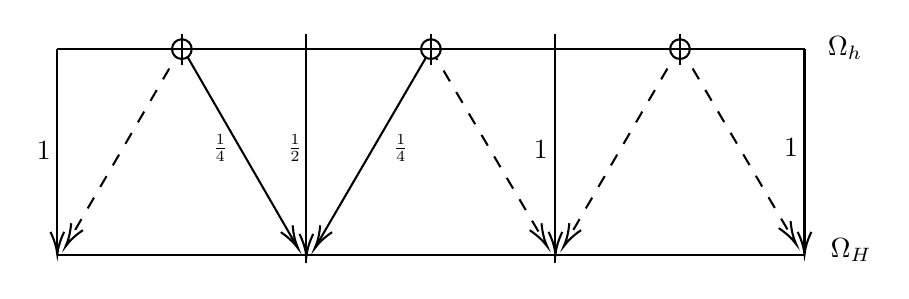
\begin{tikzpicture}[x=0.75pt,y=0.75pt,yscale=-1,xscale=1]
%uncomment if require: \path (0,138.3333282470703); %set diagram left start at 0, and has height of 138.3333282470703

%Straight Lines [id:da2880884046198069] 
\draw    (138.5,122.33) -- (498.5,122.33) (258.5,118.33) -- (258.5,126.33)(378.5,118.33) -- (378.5,126.33) ;


%Straight Lines [id:da9043200865466268] 
\draw    (138.5,23.33) -- (138.5,120.33) ;
\draw [shift={(138.5,122.33)}, rotate = 270] [color={rgb, 255:red, 0; green, 0; blue, 0 }  ][line width=0.75]    (10.93,-3.29) .. controls (6.95,-1.4) and (3.31,-0.3) .. (0,0) .. controls (3.31,0.3) and (6.95,1.4) .. (10.93,3.29)   ;

%Straight Lines [id:da008007717122758606] 
\draw  [dash pattern={on 4.5pt off 4.5pt}]  (198.5,22.33) -- (143.51,116.61) ;
\draw [shift={(142.5,118.33)}, rotate = 300.26] [color={rgb, 255:red, 0; green, 0; blue, 0 }  ][line width=0.75]    (10.93,-3.29) .. controls (6.95,-1.4) and (3.31,-0.3) .. (0,0) .. controls (3.31,0.3) and (6.95,1.4) .. (10.93,3.29)   ;

%Straight Lines [id:da8811452979136021] 
\draw    (198.5,22.33) -- (253.5,117.6) ;
\draw [shift={(254.5,119.33)}, rotate = 240] [color={rgb, 255:red, 0; green, 0; blue, 0 }  ][line width=0.75]    (10.93,-3.29) .. controls (6.95,-1.4) and (3.31,-0.3) .. (0,0) .. controls (3.31,0.3) and (6.95,1.4) .. (10.93,3.29)   ;

%Straight Lines [id:da8625316031214776] 
\draw    (258.5,24.33) -- (258.5,121.33) ;
\draw [shift={(258.5,123.33)}, rotate = 270] [color={rgb, 255:red, 0; green, 0; blue, 0 }  ][line width=0.75]    (10.93,-3.29) .. controls (6.95,-1.4) and (3.31,-0.3) .. (0,0) .. controls (3.31,0.3) and (6.95,1.4) .. (10.93,3.29)   ;

%Straight Lines [id:da6460906930372297] 
\draw    (318.5,23.33) -- (263.51,117.61) ;
\draw [shift={(262.5,119.33)}, rotate = 300.26] [color={rgb, 255:red, 0; green, 0; blue, 0 }  ][line width=0.75]    (10.93,-3.29) .. controls (6.95,-1.4) and (3.31,-0.3) .. (0,0) .. controls (3.31,0.3) and (6.95,1.4) .. (10.93,3.29)   ;

%Straight Lines [id:da8524817762946206] 
\draw  [dash pattern={on 4.5pt off 4.5pt}]  (318.5,23.33) -- (373.48,116.61) ;
\draw [shift={(374.5,118.33)}, rotate = 239.48] [color={rgb, 255:red, 0; green, 0; blue, 0 }  ][line width=0.75]    (10.93,-3.29) .. controls (6.95,-1.4) and (3.31,-0.3) .. (0,0) .. controls (3.31,0.3) and (6.95,1.4) .. (10.93,3.29)   ;

%Straight Lines [id:da8860914104807238] 
\draw    (378.5,23.33) -- (378.5,120.33) ;
\draw [shift={(378.5,122.33)}, rotate = 270] [color={rgb, 255:red, 0; green, 0; blue, 0 }  ][line width=0.75]    (10.93,-3.29) .. controls (6.95,-1.4) and (3.31,-0.3) .. (0,0) .. controls (3.31,0.3) and (6.95,1.4) .. (10.93,3.29)   ;

%Straight Lines [id:da1596911357050117] 
\draw  [dash pattern={on 4.5pt off 4.5pt}]  (438.5,22.33) -- (383.51,116.61) ;
\draw [shift={(382.5,118.33)}, rotate = 300.26] [color={rgb, 255:red, 0; green, 0; blue, 0 }  ][line width=0.75]    (10.93,-3.29) .. controls (6.95,-1.4) and (3.31,-0.3) .. (0,0) .. controls (3.31,0.3) and (6.95,1.4) .. (10.93,3.29)   ;

%Straight Lines [id:da6738060748467927] 
\draw  [dash pattern={on 4.5pt off 4.5pt}]  (438.5,22.33) -- (493.48,115.61) ;
\draw [shift={(494.5,117.33)}, rotate = 239.48] [color={rgb, 255:red, 0; green, 0; blue, 0 }  ][line width=0.75]    (10.93,-3.29) .. controls (6.95,-1.4) and (3.31,-0.3) .. (0,0) .. controls (3.31,0.3) and (6.95,1.4) .. (10.93,3.29)   ;

%Straight Lines [id:da14729734919526516] 
\draw    (498.5,23.33) -- (498.5,120.33) ;
\draw [shift={(498.5,122.33)}, rotate = 270] [color={rgb, 255:red, 0; green, 0; blue, 0 }  ][line width=0.75]    (10.93,-3.29) .. controls (6.95,-1.4) and (3.31,-0.3) .. (0,0) .. controls (3.31,0.3) and (6.95,1.4) .. (10.93,3.29)   ;

%Shape: Circle [id:dp8902650563668026] 
\draw  [fill={rgb, 255:red, 255; green, 255; blue, 255 }  ,fill opacity=1 ] (193.75,23.33) .. controls (193.75,20.71) and (195.88,18.58) .. (198.5,18.58) .. controls (201.12,18.58) and (203.25,20.71) .. (203.25,23.33) .. controls (203.25,25.96) and (201.12,28.08) .. (198.5,28.08) .. controls (195.88,28.08) and (193.75,25.96) .. (193.75,23.33) -- cycle ;
%Shape: Circle [id:dp3193149753799873] 
\draw  [fill={rgb, 255:red, 255; green, 255; blue, 255 }  ,fill opacity=1 ] (313.75,23.33) .. controls (313.75,20.71) and (315.88,18.58) .. (318.5,18.58) .. controls (321.12,18.58) and (323.25,20.71) .. (323.25,23.33) .. controls (323.25,25.96) and (321.12,28.08) .. (318.5,28.08) .. controls (315.88,28.08) and (313.75,25.96) .. (313.75,23.33) -- cycle ;
%Shape: Circle [id:dp4791222375175954] 
\draw  [fill={rgb, 255:red, 255; green, 255; blue, 255 }  ,fill opacity=1 ] (433.75,23.33) .. controls (433.75,20.71) and (435.88,18.58) .. (438.5,18.58) .. controls (441.12,18.58) and (443.25,20.71) .. (443.25,23.33) .. controls (443.25,25.96) and (441.12,28.08) .. (438.5,28.08) .. controls (435.88,28.08) and (433.75,25.96) .. (433.75,23.33) -- cycle ;
%Straight Lines [id:da8587309614827141] 
\draw    (138.5,23.33) -- (498.5,23.33) (198.5,15.83) -- (198.5,30.83)(258.5,15.83) -- (258.5,30.83)(318.5,15.83) -- (318.5,30.83)(378.5,15.83) -- (378.5,30.83)(438.5,15.83) -- (438.5,30.83) ;




% Text Node
\draw (518,23) node   {$\Omega _{h}$};
% Text Node
\draw (521,120) node   {$\Omega _{H}$};
% Text Node
\draw (253,71) node [scale=0.8]  {$\frac{1}{2}$};
% Text Node
\draw (217,71) node [scale=0.8]  {$\frac{1}{4}$};
% Text Node
\draw (304,71) node [scale=0.8]  {$\frac{1}{4}$};
% Text Node
\draw (132,72) node   {$1$};
% Text Node
\draw (371.5,71.83) node   {$1$};
% Text Node
\draw (492,71) node   {$1$};


\end{tikzpicture}

	\end{center}
	\caption{injection operator as restriction}
\end{figure}

\begin{align*}
	x^{k}- {x}^{*} &= \delta^{k}\underbrace{(x^{0}- {x}^{*})}_{e^{0}} \\
				   &=\sum_{j=1}^{n}{\delta ^{k}\xi _{j}w_{j}} \\
				   &= \sum_{j=1}^{n}{\lambda ^{k}_{j}\xi _{j}w_{j}}
\end{align*}
with
\[
e^{0} = \sum_{j=1}^{n}{\xi _{j}w_{j}}
,\] 
where $\lambda _{j} \in \sigma (G)$ and $w_{j}$ corresponding eigenvector of $\lambda _{j}$

\begin{exam} Easy Poisson
%\label{thm:}
\[
	\begin{array}{rl}
		-u''(x) = f(x) &\quad x \in (0,1) \\
		u(x) = 0 &\quad x \in \left\{ 0,1 \right\} 
	\end{array}
.\] 	
We use
\[
h = \frac{1}{n+1} \quad x_{i}= ih \quad \Omega _{h} = \left\{ x_{i} \right\} 
.\] 
What are eigenfunctions of $-\laplace$ in 1D with zero Dirichlet boundary condition on $(0,1)$?
\[
	-w''(x) = \lambda w(x)
,\] 
with
\begin{align*}
	w_{k} = \sin(k \pi x)
	\lambda _{k} = \ldots 
\end{align*}
For
\[
A = \begin{bmatrix}
	2 & -1 \\
	-1 & 2 \\
	   && \ddots \\
	   &&&2 & -1 \\
	   &&&-1 & 2
	\end{bmatrix}
\] 
we get eigenvectors for inner points
\[
w_{k} = \begin{pmatrix}
	\sin \left( \frac{1k \pi }{n+1} \right) \\
	\sin \left( \frac{2k \pi }{n+1} \right) \\
	\vdots \\
	\sin \left( \frac{nk \pi }{n+1} \right) \\
\end{pmatrix}
.\] 
associated to the eigenvalues
\[
	\lambda _{k} =  4\sin^2 \left( \frac{k \pi }{n+1} \right) 
.\] 
\end{exam}

Richardson iteration
\[
\delta _{R} = I-\omega A
.\] 
\[
	\sigma (\delta _{R}) = \left\{ 1-\omega \lambda _{k} \right\} 
.\] 
The error $e^{k}$ now reads
\[
	e^{k} = \sum_{j=1}^{n}{\underbrace{(1-\omega \lambda _{j})^{k}}_{1-4 \omega \sin^2 \left( \frac{j \pi }{n+1} \right) } \xi _{j} w_{j}}
.\] 

\begin{figure}[H]
	\begin{center}
		\tikzset{every picture/.style={line width=0.75pt}} %set default line width to 0.75pt        

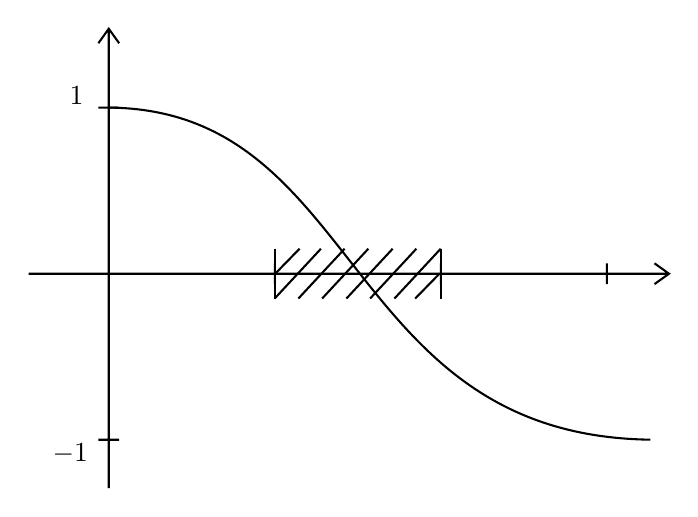
\begin{tikzpicture}[x=0.75pt,y=0.75pt,yscale=-1,xscale=1]
%uncomment if require: \path (0,240.3333282470703); %set diagram left start at 0, and has height of 240.3333282470703

%Shape: Axis 2D [id:dp8744292253516122] 
\draw  (176,128.04) -- (484.5,128.04)(214.56,10) -- (214.56,231.33) (477.5,123.04) -- (484.5,128.04) -- (477.5,133.04) (209.56,17) -- (214.56,10) -- (219.56,17) (294.56,123.04) -- (294.56,133.04)(374.56,123.04) -- (374.56,133.04)(454.56,123.04) -- (454.56,133.04)(209.56,48.04) -- (219.56,48.04)(209.56,208.04) -- (219.56,208.04) ;
\draw   ;
%Curve Lines [id:da3755881377616741] 
\draw    (214.5,48) .. controls (337.5,49) and (326.5,206) .. (475.5,208) ;



%Shape: Rectangle [id:dp05938687913112406] 
\draw  [color={rgb, 255:red, 255; green, 255; blue, 255 }  ,draw opacity=0 ] (294.5,116) -- (374.5,116) -- (374.5,140) -- (294.5,140) -- cycle ;
%Straight Lines [id:da4114855802815167] 
\draw    (294.5,140) -- (316.79,116) ;


%Straight Lines [id:da21786398588085976] 
\draw    (317.36,140) -- (339.64,116) ;


%Straight Lines [id:da5999167644642049] 
\draw    (305.93,140) -- (328.21,116) ;


%Straight Lines [id:da5887247610166593] 
\draw    (329.07,140) -- (351.36,116) ;


%Straight Lines [id:da9800992774415527] 
\draw    (340.5,140) -- (362.79,116) ;


%Straight Lines [id:da4509788472444165] 
\draw    (352.21,140) -- (374.5,116) ;


%Straight Lines [id:da7403253143757675] 
\draw    (362.21,140) -- (373.93,128) ;


%Straight Lines [id:da32294781199370126] 
\draw    (294.79,128) -- (306.5,116) ;


%Straight Lines [id:da36702102584283813] 
\draw [color={rgb, 255:red, 0; green, 0; blue, 0 }  ,draw opacity=1 ]   (294.5,116) -- (294.5,140) ;


%Straight Lines [id:da7570534048443951] 
\draw [color={rgb, 255:red, 0; green, 0; blue, 0 }  ,draw opacity=1 ]   (374.5,116) -- (374.5,140) ;




% Text Node
\draw (199,42) node   {$1$};
% Text Node
\draw (196,215) node   {$-1$};


\end{tikzpicture}

	\end{center}
	\caption{sketch for $\omega = \frac{1}{2}$}
	\label{fig:}
\end{figure}

\begin{figure}[H]
	\begin{center}
		\tikzset{every picture/.style={line width=0.75pt}} %set default line width to 0.75pt        

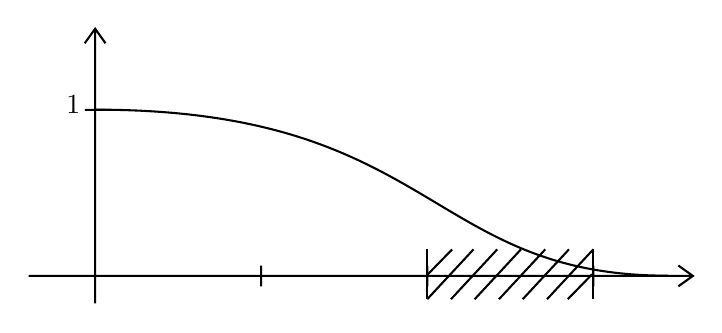
\begin{tikzpicture}[x=0.75pt,y=0.75pt,yscale=-1,xscale=1]
%uncomment if require: \path (0,152.66665649414062); %set diagram left start at 0, and has height of 152.66665649414062

%Shape: Axis 2D [id:dp8270164404623155] 
\draw  (170.5,129.77) -- (490.5,129.77)(202.5,10.67) -- (202.5,143) (483.5,124.77) -- (490.5,129.77) -- (483.5,134.77) (197.5,17.67) -- (202.5,10.67) -- (207.5,17.67) (282.5,124.77) -- (282.5,134.77)(362.5,124.77) -- (362.5,134.77)(442.5,124.77) -- (442.5,134.77)(197.5,49.77) -- (207.5,49.77) ;
\draw   ;
%Curve Lines [id:da26521574633074274] 
\draw    (202.5,49.67) .. controls (366.5,49.67) and (362.5,129.67) .. (478.5,129.67) ;


%Shape: Rectangle [id:dp07766955074375792] 
\draw  [color={rgb, 255:red, 255; green, 255; blue, 255 }  ,draw opacity=0 ] (362.5,117) -- (442.5,117) -- (442.5,141) -- (362.5,141) -- cycle ;
%Straight Lines [id:da4312858915297626] 
\draw    (362.5,141) -- (384.79,117) ;


%Straight Lines [id:da5542417692050874] 
\draw    (385.36,141) -- (407.64,117) ;


%Straight Lines [id:da17968044358338675] 
\draw    (373.93,141) -- (396.21,117) ;


%Straight Lines [id:da018335299880271716] 
\draw    (397.07,141) -- (419.36,117) ;


%Straight Lines [id:da5204059688682119] 
\draw    (408.5,141) -- (430.79,117) ;


%Straight Lines [id:da3294948143034826] 
\draw    (420.21,141) -- (442.5,117) ;


%Straight Lines [id:da3684546422227106] 
\draw    (430.21,141) -- (441.93,129) ;


%Straight Lines [id:da5208205652283249] 
\draw    (362.79,129) -- (374.5,117) ;


%Straight Lines [id:da26320261899336517] 
\draw [color={rgb, 255:red, 0; green, 0; blue, 0 }  ,draw opacity=1 ]   (362.5,117) -- (362.5,141) ;


%Straight Lines [id:da20937537573033715] 
\draw [color={rgb, 255:red, 0; green, 0; blue, 0 }  ,draw opacity=1 ]   (442.5,117) -- (442.5,141) ;





% Text Node
\draw (192,47) node   {$1$};


\end{tikzpicture}

	\end{center}
	\caption{sketch for $\omega = \frac{1}{4}$}
	\label{fig:}
\end{figure}
